\documentclass[12pt]{article}
\usepackage[margin=1in]{geometry}
\usepackage{setspace}
\onehalfspacing{}
\usepackage[dvipsnames,table,xcdraw]{xcolor} % colors

% Start of preamble
%==========================================================================================%
% Required to support mathematical unicode
\usepackage[warnunknown, fasterrors, mathletters]{ucs}
\usepackage[utf8x]{inputenc}

% Standard mathematical typesetting packages
\usepackage{amsmath,amssymb,amscd,amsthm,amsxtra, newtxtext, newtxmath}
\usepackage{mathtools,mathrsfs,xparse}

% Symbol and utility packages
\usepackage{cancel, textcomp}
\usepackage[mathscr]{euscript}
\usepackage[nointegrals]{wasysym}
\usepackage{apacite}

% Extras
\usepackage{physics}  % Lots of useful shortcuts and macros
\usepackage{tikz-cd}  % For drawing commutative diagrams easily
\usepackage{microtype}  % Minature font tweaks
%\usepackage{pgfplots} % plots

\usepackage{enumitem}
\usepackage{titling}

\usepackage{graphicx}

%\usepackage{quiver}

% Fancy theorems due to @intuitively on discord
\usepackage{mdframed}
\newmdtheoremenv[
backgroundcolor=NavyBlue!30,
linewidth=2pt,
linecolor=NavyBlue,
topline=false,
bottomline=false,
rightline=false,
innertopmargin=10pt,
innerbottommargin=10pt,
innerrightmargin=10pt,
innerleftmargin=10pt,
skipabove=\baselineskip,
skipbelow=\baselineskip]{mytheorem}{Theorem}

\newenvironment{theorem}{\begin{mytheorem}}{\end{mytheorem}}

\newtheorem{corollary}{Corollary}
\newtheorem{lemma}{Lemma}

\newtheoremstyle{definitionstyle}
{\topsep}%
{\topsep}%
{}%
{}%
{\bfseries}%
{.}%
{.5em}%
{}%
\theoremstyle{definitionstyle}
\newmdtheoremenv[
backgroundcolor=Violet!30,
linewidth=2pt,
linecolor=Violet,
topline=false,
bottomline=false,
rightline=false,
innertopmargin=10pt,
innerbottommargin=10pt,
innerrightmargin=10pt,
innerleftmargin=10pt,
skipabove=\baselineskip,
skipbelow=\baselineskip,
]{mydef}{Definition}
\newenvironment{definition}{\begin{mydef}}{\end{mydef}}

\newtheorem*{remark}{Remark}

\newtheorem*{example}{Example}
\newtheorem*{claim}{Claim}

% Common shortcuts
\def\mbb#1{\mathbb{#1}}
\def\mfk#1{\mathfrak{#1}}

\def\bN{\mbb{N}}
\def\C{\mbb{C}}
\def\R{\mbb{R}}
\def\bQ{\mbb{Q}}
\def\bZ{\mbb{Z}}
\def\cph{\varphi}
\renewcommand{\th}{\theta}
\def\ve{\varepsilon}
\newcommand{\mg}[1]{\| #1 \|}

% Often helpful macros
\newcommand{\floor}[1]{\left\lfloor#1\right\rfloor}
\newcommand{\ceil}[1]{\left\lceil#1\right\rceil}
\renewcommand{\qed}{\hfill\qedsymbol}
\renewcommand{\ip}[1]{\langle#1\rangle}
\newcommand{\seq}[2]{\qty(#1_#2)_{#2=1}^{\infty}}

\newcommand{\SET}[1]{\Set{\mskip-\medmuskip #1 \mskip-\medmuskip}}

% End of preamble
%==========================================================================================%

% Start of commands specific to this file
%==========================================================================================%

\usepackage{braket}
\newcommand{\Z}{\mbb Z}
\newcommand{\gen}[1]{\left\langle #1 \right\rangle}
\newcommand{\nsg}{\trianglelefteq}
\newcommand{\F}{\mbb F}
\newcommand{\Aut}{\mathrm{Aut}}
\newcommand{\sepdeg}[1]{[#1]_{\mathrm{sep}}}
\newcommand{\Q}{\mbb Q}
\newcommand{\Gal}{\mathrm{Gal}\qty}
\newcommand{\id}{\mathrm{id}}
\newcommand{\Hom}{\mathrm{Hom}_R}
\newcommand{\1}{\mathds 1}
\newcommand{\N}{\mathbb N}
\renewcommand{\P}{\mathbb P \qty}
\newcommand{\E}{\mathbb E \qty}
\newcommand{\Var}{\mathrm{Var}}
\everymath{\displaystyle}
\newcommand{\argmax}{\mathrm{argmax}}

%==========================================================================================%
% End of commands specific to this file

\title{Math 522 HW2}
\date{\today}
\author{Rohan Mukherjee, Alex Albors, Victor Krassovsky}

\begin{document}
    \maketitle
    \subsection*{Problem 4.4.7.}
    The next result gives an extension of Theorem 4.4.2 to $p = 1$. Let $X_n$ be a martingale with $X_0 = 0$ and $E X_n^2 < \infty$. Show that
    \begin{align*}
        P(\max_{m \leq n} X_m \geq \lambda) \leq E X_n^2 / (E X_n^2 + \lambda^2)
    \end{align*}

    Let $c$ be a constant to be chosen later. $X_n + c$ is a martingale, and since $x^2$ is convex $(X_n+c)^2$ is a submartingale. Thus by Doob's inequality, we have that:
    \begin{align*}
        \P(\max_{m \leq n} X_m \geq \lambda) \leq \P(\max_{m \leq n} (X_m + c)^2 \geq (\lambda+c)^2) \leq \frac{E\qty((X_n+c)^2)}{(\lambda+c)^2}
    \end{align*}
    Notice that $E\qty((X_n+c)^2) = E X_n^2 + 2c E X_n + c^2$. Since $X_n$ is a martingale with $X_0 = 0$, we know that $E X_n = 0$ for all $n$, and hence $E\qty((X_n+c)^2) = E X_n^2 + c^2$. Thus, we have:
    \begin{align*}
        \P(\max_{m \leq n} X_m \geq \lambda) \leq \frac{E X_n^2 + c^2}{(\lambda+c)^2}
    \end{align*}
    The  derivative of the RHS is just:
    \begin{align*}
        \frac{2(\lambda + c)(E X_n^2 + c^2) - 2c (\lambda + c)^2}{(\lambda+c)^4}
    \end{align*}
    Setting this equal to 0 we find that $c = E X_n^2 / \lambda$ is a minimizer. Plugging this back in:
    \begin{align*}
        \P(\max_{m \leq n} X_m \geq \lambda) &\leq \frac{E X_n^2 + \qty(\frac{E X_n^2}{\lambda})^2}{(\lambda + \frac{E X_n^2}{\lambda})^2} = \frac{\lambda^2EX_n^2 + \qty(E X_n^2)^2}{(\lambda^2 + E X_n^2)^2} 
        \\&= \frac{E X_n^2}{E X_n^2 + \lambda^2}.
    \end{align*}

    \subsection*{Problem 4.6.2.}
    $f$ is said to be \textbf{Lipschitz continuous} if $|f(t) - f(s)| \leq L|t-s|$ for $0 \leq s,t < 1$. Show that $X_n = 2^n (f((k+1)/2^n) - f(k/2^n))$ on $I_{k,n} = \qty[k/2^n, (k+1)/2^n]$ defines a martingale, $X_n \to X_\infty$ a.s. and in $L^1$, and 
    \begin{align*}
        f(b) - f(a) = \int_a^b X_\infty(\omega) d\omega
    \end{align*}
    for every $a < b$.

    Recall that $\mathcal F_n = \sigma(I_{k,n} : 0 \leq k < 2^n)$. Firstly, $E(X_{n+1} \mid \mathcal F_n)$ is constant on each of the $I_{k,n}$ by a result we proved in class, namely that if $\SET{U_i}_i$ is a sequence of disjoint sets whose union is $\Omega$, then $\sigma(U_i : i \in \N)$ is just disjoint unions of the $U_i$. In particular, $I_{k,n}$ is the finest set in $\mathcal F_n$, so $E(X_{n+1} \mid \mathcal F_n)$ is constant on each $I_{k,n}$. By the conditional expectation,
    \begin{align*}
        E(1_{I_{k,n}}E(X_{n+1} \mid \mathcal F_n)) &= E(1_{I_{k,n}}X_{n+1}) 
        \\&= f((2k+2)/2^{n+1}) - f((2k+1)/2^{n+1}) + f((2k+1)/2^{n+1}) - f(2k/2^{n+1}) 
        \\&= f((k+1)/2^n) - f(k/2^n)
    \end{align*}
    Since $I_{k,n}$ has measure $1/2^n$, this shows that $E(X_{n+1} \mid \mathcal F_n) = X_n$. Thus, $X_n$ is a martingale. Further, on $I_{k,n}$,
    \begin{align*}
        |X_n| = |2^n (f((k+1)/2^n) - f(k/2^n))| \leq L
    \end{align*}
    by the Lipschitz continuity of $f$. So $|X_n|$ is bounded, and in particular $\SET{X_n}_n$ is uniformly integrable. Thus $X_n \to X_\infty$ a.s. and in $L^1$ (By Theorem 4.6.4).

    Now, for $a < b$, and a fixed $n$, find $k,l$ satisfying $k/2^n \leq a < (k+1)/2^n$, $l/2^n \leq b < (l+1)/2^n$. Then we have:

    \begin{center}
        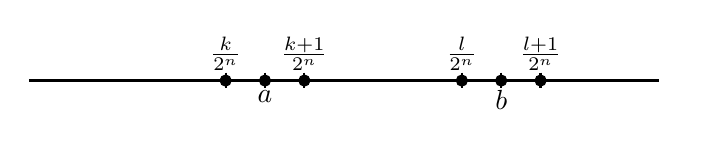
\begin{tikzpicture}
            % Draw number line
            \draw[thick, -] (-4,0) -- (4,0) node[right] {};

            % Points and labels
            \filldraw[black] (-1.5,0) circle (2pt) node[above] {$\frac{k}{2^n}$};
            \filldraw[black] (-1,0) circle (2pt) node[below] {$a$};
            \filldraw[black] (-0.5,0) circle (2pt) node[above] {$\frac{k+1}{2^n}$};
            
            \filldraw[black] (1.5,0) circle (2pt) node[above] {$\frac{l}{2^n}$};
            \filldraw[black] (2,0) circle (2pt) node[below] {$b$};
            \filldraw[black] (2.5,0) circle (2pt) node[above] {$\frac{l+1}{2^n}$};

            % Small gaps for clarity
            \draw[thick] (-1.5,0.1) -- (-1.5,-0.1);
            \draw[thick] (-1,0.1) -- (-1,-0.1);
            \draw[thick] (-0.5,0.1) -- (-0.5,-0.1);

            \draw[thick] (1.5,0.1) -- (1.5,-0.1);
            \draw[thick] (2,0.1) -- (2,-0.1);
            \draw[thick] (2.5,0.1) -- (2.5,-0.1);
        \end{tikzpicture}
    \end{center}
    Since $X_n \to X_\infty$ in $L^1$, we have $E(X_n 1_{(a,b)}) \to E(X_\infty 1_{(a,b)})$ for every $a < b$. By running the telescoping series, we can see that:
    \begin{align*}
        E(X_n 1_{(a,b)}) &= \qty[f((l+1)/2^n) - f(k/2^n)] - \qty[f((l+1)/2^n) - f(l/2^n)]2^n ((l+1)/2^n - b) \\
        & - \qty[f((k+1)/2^n) - f(k/2^n)] 2^n (a - k/2^n)
    \end{align*}
    Now notice that, by Lipschitz,
    \begin{align*}
        |\qty[f((l+1)/2^n) - f(l/2^n)]2^n ((l+1)/2^n - b)| \leq L/2^n
    \end{align*}
    and,
    \begin{align*}
        |\qty[f((k+1)/2^n) - f(k/2^n)] 2^n (a - k/2^n)| \leq L/2^n
    \end{align*}
    Further,
    \begin{align*}
        \qty[f((l+1)/2^n) - f(k/2^n)] + \qty[f((l+1)/2^n) - f(b)] + [f(a) - f(k/2^n)]
    \end{align*}
    With:
    \begin{align*}
        |[f((l+1)/2^n) - f(b)]| , |[f(a) - f(k/2^n)]| \leq L/2^n
    \end{align*}
    Thus,
    \begin{align*}
        |E(X_n 1_{(a,b)}) - (f(b)-f(a))| \leq L/2^{n-2}
    \end{align*}
    We conclude that $E(X_\infty 1_{(a,b)}) = f(b) - f(a)$. I believe this is related to Lipschitz continuity implying differentiable a.e.

    \subsection*{Problem 4.6.6.}
    Let $X_n \in [0,1]$ be adapted to $\mathcal F_n$. Let $\alpha, \beta > 0$ with $\alpha + \beta = 1$ and suppose
    \begin{align*}
        P(X_{n+1} = \alpha + \beta X_n \mid \mathcal F_n) = X_n \quad P(X_{n+1} = \beta X_n \mid \mathcal F_n) = 1 - X_n
    \end{align*}
    Show $P(\lim X_n = 0 \text{ or } 1) = 1$ and if $E(X_0) = \theta$ then $P(\lim X_n = 1) = \theta$.

    \textbf{Proof.} 
    We show that $X_n$ is a martingale. Indeed, 
    \begin{align*}
        E(X_{n+1} \mid \mathcal F_n) = (\alpha + \beta X_n) X_n + \beta X_n (1-X_n) = (\alpha + \beta)X_n = X_n
    \end{align*}
    Further, since $X_n \in [0,1]$, it is bounded, hence uniformly integrable, so it converges a.s. and in $L^1$ to some $X = \lim X_n$. Since $X_{n+1} = \alpha + \beta X_n$ or $\beta X_n$ a.s., either the first case happens infinitely often or the second does. In the first case, for infinitely many $n$,
    \begin{align*}
        X_{n+1} = \alpha + \beta X_n + \alpha X_n - \alpha X_n = \alpha + X_n - \alpha X_n
    \end{align*}
    So,
    \begin{align*}
        |X_{n+1} - X_n| = \alpha |1 - X_n|
    \end{align*}
    Since the sequence converges, it is Cauchy, so we have found a subsequence converging to 1. Since the whole sequence converges, any subsequence must converge to the same value, so in this case $X_n \to 1$. In the second case,
    \begin{align*}
        X_{n+1} = \beta X_n + \alpha X_n - \alpha X_n = X_n - \alpha X_n
    \end{align*}
    So we find infinitely many $n$s satisfying:
    \begin{align*}
        |X_{n+1} - X_n| = \alpha |X_n|
    \end{align*}
    This yields a subsequence tending to 0, so the entire sequence goes to 0. 

    From this, since $X$ only takes the values 0,1 almost surely, we know that:
    \begin{align*}
        E(X) = P(X = 1)
    \end{align*}
    Finally, since $X_n \to X$ in $L^1$, we have that:
    \begin{align*}
        \theta = E(X_0) = \lim_n E(X_n) = E(X) = P(X = 1).
    \end{align*}

    \subsection*{Problem 4.8.5.} \textit{Variance of the gambler's ruin.} Let $\xi_1, \xi_2, \ldots$ be independent with $P(\xi_i = 1) = p$ and $P(\xi_i = -1) = q = 1-p$ where $p < 1/2$. Let $S_n = x + \xi_1 + \cdots + \xi_n$ and let $V_0 = \inf \SET{n \geq 0 : S_n = 0}$. Theorem 4.8.9 tells us that $E_x V_0 = x/(1-2p)$. The aim of this problem is to compute the variance of $V_0$. if we let $Y_i = \xi_i - (p-q)$ and note that $E Y_i = 0$ and 
    \begin{align*}
        \Var(Y_i) = \Var(X_i) = E X_i^2 - (E X_i)^2
    \end{align*}
    then it follows that $M_n = (S_n - (p-q)n)^2 - n(1-(p-q)^2)$ is a martingale. 

    (a) Use this to conclude that when $S_0 = x$, the variance of $V_0$ is 
    \begin{align*}
        x \cdot \frac{1 - (p-q)^2}{(q-p)^3}
    \end{align*}

    (b) Why must the answer in (a) be of the form $cx$?
    
    \textbf{Solution.}
    (a) We write $S_n = \xi_1 + \cdots + \xi_n$ and let $V_x = \inf \SET{n \geq 0 : S_n = -x}$. Applying theorem 4.4.1 to $M_n = (S_n - (p-q)n)^2 - n(1-(p-q)^2)$, we have:
    \begin{align*}
        E(S_{n \land V_x} - (p-q)(n \land V_x))^2 = (1-(p-q)^2)E(V_x \land n)
    \end{align*}
    Obviously, $E(V_x \land n) \leq E(V_x) = x/(q-p) < \infty$. Thus $E(S_{n \land V_x} - (p-q)(n \land V_x))^2$ is bounded in $L^2$ and hence it converges in $L^2$ (BY MAGIC). Thus,
    \begin{align*}
        E(S_{V_x} - (p-q)V_x)^2 = (1-(p-q)^2)E(V_x) = x\frac{(1-(p-q)^2)}{q-p}
    \end{align*}
    Simultaneously, since $S_{V_x} = -x$,
    \begin{align*}
        E(S_{V_x} - (p-q)V_x)^2 = x^2 + 2x(p-q)E(V_x) + (p-q)^2E(V_x^2)
    \end{align*}
    Some algebra shows that
    \begin{align*}
        E(V_x^2) = x \frac{1-(p-q)^2}{(q-p)^3} + \frac{x^2}{(p-q)^2}
    \end{align*}
    We conclude that
    \begin{align*}
        \Var(V_x) = x\frac{1-(p-q)^2}{(q-p)^3}.
    \end{align*}


    (b) Let $S_n$ start at 0 and $V_0^x = \inf \SET{n \geq 0 : S_n = x}$ for each $x$. If we let $\hat S_n$ be an independent copy of $S_n$, and $\hat V_0^{y}$ its hitting time, then I claim that $V_0^{x+y}$ has the same distribution as $V_0^x + \hat V_0^{y}$. Indeed,
    \begin{align*}
        P(V_0^{x+y} = m) &= \sum_{n \leq m} P(V_0^{x+y} = m \mid V_0^x = n) P(V_0^x = n) \\
        &= \sum_{n \leq m} P(S_{n+1} \neq x+y, \ldots, S_m = x+y \mid V_0^x = n)P(V_0^x = n) \\
        &= \sum_{n \leq m} P(S_{n+1} - S_n \neq y, \ldots, S_m - S_n = y \mid V_0^x = n)P(V_0^x = n)
    \end{align*}
    From here, $\SET{V_0^x = n}$ is $\mathcal F_n$ measurable, while $S_{n+1} - S_n, \ldots, S_m - S_n$ are independent of $\mathcal F_n$. Thus,
    \begin{align*}
        P(V_0^{x+y} = m) &= \sum_{n \leq m} P(S_{n+1} - S_n \neq y, \ldots, S_m - S_n = y)P(V_0^x = n) \\
        &= \sum_{n \leq m} P(\hat S_1 \neq y, \ldots, \hat S_{m-n} = y)P(V_0^x = n) \\
        &= \sum_{n \leq m} P(\hat V_0^y = m-n)P(V_0^x = n) = P(V_0^x + \hat V_0^y = m)
    \end{align*}
    In particular, $\Var(V^{x+y}_0) = \Var(V_0^x + \hat V_0^y) = \Var(V_0^x) + \Var(V_0^y)$. This shows that $f(x+y) = f(x) + f(y)$, which means that $f(x) = cx$.

    \subsection*{Problem 4.8.7.}
    Let $S_n$ be a symmetric simple random walk starting at 0, and let $T = \inf\SET{n : S_n \not \in (-a,a)}$ where $a$ is an integer. Find constants $b,c$ so that $Y_n = S_n^4 - 6nS_n^2 + bn^2 + cn$ is a martingale, and use this to compute $ET^2$.

    \textbf{Solution.}
    We compute:
    \begin{align*}
        E(Y_{n+1} \mid \mathcal F_n) &= E(S_n^4 + 4S_n^3\xi_{n+1} + 6S_n^2\xi_{n+1}^2 + 4S_n\xi_{n+1}^3 + \xi_{n+1}^4 
        \\ &- 6(n+1)(S_n^2 + 2\xi_{n+1}S_n + \xi_{n+1}^2) + b(n+1)^2 + c(n+1) \mid \mathcal F_n) \\
        &= E(S_n^4 + 6S_n^2 + 1 - 6(n+1)(S_n^2 + 1) + b(n+1)^2 + c(n+1) \mid \mathcal F_n) \\
        &= E(S_n^4 + 6S_n^2 + 1 - 6nS_n^2 - 6S_n^2 - 6n - 6 + bn^2 + 2bn + b + cn + c \mid \mathcal F_n) \\
        &= Y_n - 6n + 2bn + b + c -5
    \end{align*}
    So we need $b = 3$ and $c = 2$. Recall from the book that $ET = a^2$. By applying Theorem 4.4.1 to the bounded stopping time $T \land n$, we get:
    \begin{align*}
        E(S_{n \land T}^4 - 6(n \land T) S_{n \land T}^2 + 3(n \land T)^2 + 2(n \land T)) = 0
    \end{align*}
    The monotone convergence theorem shows that $E(n \land T) \to E(T)$ and $E(n \land T)^2 \to E(T^2)$. Since $S_{n \land T}^4 \leq a^4$, it is bounded, so by the bounded convergence theorem we have $E(S_{n \land T}^4) \to E(S_T^4) = a^4$. As $|(n \land T)S_{n \land T}^2| \leq a^2T$, dominated convergence theorem shows that $E((n \land T)S_{n \land T}) \to E(TS_T^2) = a^2E(T)$. Thus, we have:
    \begin{align*}
        a^4 - 6a^4 + 3E(T^2) + 2a^2 = 0
    \end{align*}
    So,
    \begin{align*}
        E(T^2) = \frac{5a^4-2a^2}{3}.
    \end{align*}

    \subsection*{Problem 2.}
    Azuma-Hoeffding inequality: Let $\SET{(X_n,\mathcal F_n); n \geq 0}$ be a martingale such that for every $k \geq 1$ $\xi_k \leq X_k - X_{k-1} \leq \xi_k + d_k$ for some constant $d_k > 0$ and random variable $\xi_k$ that is $\mathcal F_{k-1}$-measurable. Prove that for $n \geq 1$, and $\lambda > 0$,
    \begin{align*}
        P(|X_n - X_0| \geq \lambda) \leq 2\exp(-2\lambda^2\bigg/\sum_{k=1}^n d_k^2).
    \end{align*}
    
    \textbf{Solution.}
    Recall Hoeffding's lemma: If $X$ is a random variable such that $a \leq X \leq b$ almost surely, then for any $\alpha > 0$,
    \begin{align*}
        E\exp(\alpha X) \leq \exp\qty(\frac{\alpha^2(b-a)^2}{8}).
    \end{align*}
    Using this, we can write:
    \begin{align*}
        P(X_n - X_0 \geq \lambda) &= P\qty(e^{\alpha(X_n - X_0)} \geq e^{\alpha \lambda}) \leq e^{-\alpha \lambda} E e^{\alpha(X_n - X_0)}
    \end{align*}
    Now,
    \begin{align*}
        E(e^{\alpha(X_n - X_0)}) &= E(E(e^{\alpha(\sum_{k=1}^n X_k - X_{k-1})} \mid \mathcal F_{n-1})) \\
        &= E(e^{\alpha(\sum_{k=1}^{n-1} X_k - X_{k-1})} E(e^{\alpha(X_n - X_{n-1})} \mid \mathcal F_{n-1}))
    \end{align*}
    Now, $\xi_{n-1}$ is constant when conditioned on $\mathcal F_{n-1}$. So we can apply Hoeffding's lemma, and we get:
    \begin{align*}
        E(e^{\alpha(X_n - X_{n-1})} \mid \mathcal F_{n-1}) \leq \exp\qty(\frac{\alpha^2d_{n}^2}{8})
    \end{align*}
    Applying this repeatedly gives:
    \begin{align*}
        E(e^{\alpha(X_n - X_0)}) \leq \exp\qty(\frac{\alpha^2}{8}\sum_{k=1}^n d_k^2)
    \end{align*}
    Thus, for every $\alpha$,
    \begin{align*}
        P(X_n - X_0 \geq \lambda) \leq \exp\qty(-\alpha \lambda + \frac{\alpha^2}{8}\sum_{k=1}^n d_k^2)
    \end{align*}
    Optimizing over $\alpha$ yields $\alpha = 4\lambda\big/\sum_{k=1}^n d_k^2$, and plugging this back in yields:
    \begin{align*}
        P(X_n - X_0 \geq \lambda) \leq \exp\qty(-2\lambda^2\bigg/\sum_{k=1}^n d_k^2)
    \end{align*}
\end{document}